% questions.tex —— 2019 年·北京卷·文科 · 题目内容片段（无答案）
% 由 tools/generate_projects.py 依来源总账自 2019/2019_数学真题_北京卷文_试题.md 生成，勿手改（改源 MD 后重跑）

\begin{gktip}
来源：固定来源 \texttt{src-7f7753913867f6f28d3a208c66f0a0a0beea9ece56504daff36cc2faab5de57e}（\texttt{普通高考/2019/2019北京文.pdf}，原卷印刷页 1089—1090）。
声明：内部绑定只固定输入字节，不认证出版者、版次、上游来源链及官方身份；固定源不附答案页。
\end{gktip}

\par\medskip

\gkpart{一、选择题（本大题共 8 小题，每小题 5 分，共 40 分。在每小题列出的四个选项中，选出符合题目要求的一项）}

\begin{question}
\gkti{1}
已知集合 $A = \{x \mid -1 < x < 2\}$, $B = \{x \mid x > 1\}$, 则 $A \cup B =$（ ）。

(A) $(-1, 1)$　(B) $(1, 2)$　(C) $(-1, +\infty)$　(D) $(1, +\infty)$

\end{question}
\begin{question}
\gkti{2}
已知复数 $z = 2 + \mathrm{i}$, 则 $z \cdot \bar{z} =$（ ）。

(A) $\sqrt{3}$　(B) $\sqrt{5}$　(C) $3$　(D) $5$

\end{question}
\begin{question}
\gkti{3}
下列函数中, 在区间 $(0, +\infty)$ 上单调递增的是（ ）。

(A) $y = x^{\frac{1}{2}}$　(B) $y = 2^{-x}$　(C) $y = \log_{\frac{1}{2}} x$　(D) $y = \dfrac{1}{x}$

\Needspace{0.4\textheight}
\end{question}
\begin{question}
\gkti{4}
执行如图所示的程序框图, 输出的 $s$ 值为（ ）。
\nopagebreak[4]
\begin{center}\begin{tikzpicture}[>=latex, font=\small, scale=0.9]
  \tikzstyle{startstop} = [draw, rounded corners=8pt, minimum width=1.8cm, minimum height=0.65cm, text centered]
  \tikzstyle{io} = [draw, trapezium, trapezium left angle=70, trapezium right angle=110, minimum width=1.8cm, minimum height=0.65cm, text centered]
  \tikzstyle{process} = [draw, minimum width=2.0cm, minimum height=0.65cm, text centered]
  \tikzstyle{decision} = [draw, diamond, aspect=2, minimum width=2.2cm, minimum height=0.75cm, text centered]
  \tikzstyle{arrow} = [thick, ->]

  \node (start) [startstop] at (0, 0) {开始};
  \node (init) [process] at (0, -1.0) {$k = 1,\ s = 1$};
  \node (proc) [process] at (0, -2.2) {$s = \dfrac{2s^2}{3s - 2}$};
  \node (dec) [decision] at (0, -3.5) {$k \geqslant 3$?};
  \node (out) [io] at (0, -4.8) {输出 $s$};
  \node (stop) [startstop] at (0, -5.7) {结束};
  \node (inc) [process] at (2.2, -2.85) {$k = k + 1$};

  \draw[arrow] (start) -- (init);
  \draw[arrow] (init) -- (proc);
  \draw[arrow] (proc) -- (dec);
  \draw[arrow] (dec) -- node[right] {是} (out);
  \draw[arrow] (out) -- (stop);

  \draw[arrow] (dec.east) -| node[above, pos=0.25] {否} (inc.south);
  \draw[arrow] (inc.north) |- ([yshift=0.3cm]proc.north);
\end{tikzpicture}
\end{center}
\nopagebreak[4]
(A) $1$　(B) $2$　(C) $3$　(D) $4$

\end{question}
\begin{question}
\gkti{5}
已知双曲线 $\dfrac{x^2}{a^2} - y^2 = 1$ ($a > 0$) 的离心率是 $\sqrt{5}$, 则 $a =$（ ）。

(A) $\sqrt{6}$　(B) $4$　(C) $2$　(D) $\dfrac{1}{2}$

\end{question}
\begin{question}
\gkti{6}
设函数 $f(x) = \cos x + b \sin x$ ($b$ 为常数), 则“$b = 0$”是“$f(x)$ 为偶函数”的（ ）。

(A) 充分而不必要条件　(B) 必要而不充分条件
(C) 充分必要条件　(D) 既不充分也不必要条件

\end{question}
\begin{question}
\gkti{7}
在天文学中, 天体的明暗程度可以用星等或亮度来描述. 两颗星的星等与亮度满足 $m_2 - m_1 = \dfrac{5}{2}\lg \dfrac{E_1}{E_2}$, 其中星等为 $m_k$ 的星的亮度为 $E_k$ ($k = 1, 2$). 已知太阳的星等是 $-26.7$, 天狼星的星等是 $-1.45$, 则太阳与天狼星的亮度的比值为（ ）。

(A) $10^{10.1}$　(B) $10.1$　(C) $\lg 10.1$　(D) $10^{-10.1}$

\Needspace{0.4\textheight}
\end{question}
\begin{question}
\gkti{8}
如图, $A, B$ 是半径为 $2$ 的圆周上的定点, $P$ 为圆周上的动点, $\angle APB$ 是锐角, 大小为 $\beta$. 图中阴影区域的面积的最大值为（ ）。
\nopagebreak[4]
\begin{center}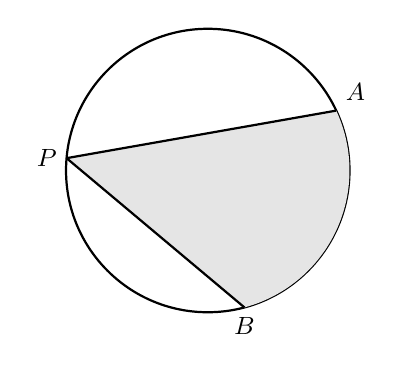
\begin{tikzpicture}[>=latex, font=\small, scale=1.0]
  \coordinate (O) at (0, 0);
  \draw[thick] (O) circle (1.8cm);

  \coordinate (P) at (175:1.8);
  \coordinate (A) at (25:1.8);
  \coordinate (B) at (285:1.8);

  % 阴影区域：弦 PA、PB 及右侧圆弧围成的区域
  \fill[gray!20] (P) -- (A) arc (25:-75:1.8cm) -- cycle;

  \draw[thick] (P) -- (A);
  \draw[thick] (P) -- (B);

  \node[left] at (P) {$P$};
  \node[above right] at (A) {$A$};
  \node[below] at (B) {$B$};
\end{tikzpicture}
\end{center}
\nopagebreak[4]
(A) $4\beta + 4\cos\beta$　(B) $4\beta + 4\sin\beta$　(C) $2\beta + 2\cos\beta$　(D) $2\beta + 2\sin\beta$

\par\medskip

\end{question}
\gkpart{二、填空题（本大题共 6 小题，每小题 5 分，共 30 分）}

\begin{question}
\gkti{9}
已知向量 $\vec{a} = (-4, 3)$, $\vec{b} = (6, m)$, 且 $\vec{a} \perp \vec{b}$, 则 $m =$ \gkblank{}。

\end{question}
\begin{question}
\gkti{10}
若 $x, y$ 满足 $\begin{cases} x \leqslant 2, \\ y \geqslant -1, \\ 4x - 3y + 1 \geqslant 0, \end{cases}$ 则 $y - x$ 的最小值为 \gkblank{}，最大值为 \gkblank{}。

\end{question}
\begin{question}
\gkti{11}
设抛物线 $y^2 = 4x$ 的焦点为 $F$, 准线为 $l$. 则以 $F$ 为圆心, 且与 $l$ 相切的圆的方程为 \gkblank{}。

\Needspace{0.4\textheight}
\end{question}
\begin{question}
\gkti{12}
某几何体是由一个正方体去掉一个四棱柱所得, 其三视图如图所示. 如果网格纸上小正方形的边长为 $1$, 那么该几何体的体积为 \gkblank{}。
\nopagebreak[4]
\begin{center}\begin{tikzpicture}[>=latex, scale=0.45, font=\small]
  % 网格底图
  \draw[step=1, gray!50, very thin] (0, -1) grid (14, 10);

  % 正 (主) 视图
  \draw[thick] (2, 5) rectangle (6, 9);
  \draw[thick] (2, 6) -- (6, 6);
  \node[below] at (4, 4.8) {正 (主) 视图};

  % 侧 (左) 视图
  \draw[thick] (9, 5) -- (13, 5) -- (13, 6) -- (11, 6) -- (9, 9) -- cycle;
  \node[below] at (11, 4.8) {侧 (左) 视图};

  % 俯视图
  \draw[thick] (2, 0) rectangle (6, 4);
  \draw[thick] (2, 2) -- (6, 2);
  \node[below] at (4, -0.2) {俯视图};
\end{tikzpicture}
\end{center}
\nopagebreak[4]
\end{question}
\begin{question}
\gkti{13}
已知 $l, m$ 是平面 $\alpha$ 外的两条不同直线. 给出下列三个论断:
① $l \perp m$;
② $m \parallel \alpha$;
③ $l \perp \alpha$.
以其中的两个论断作为条件, 余下的一个论断作为结论, 写出一个正确的命题: \gkblank{}。

\end{question}
\begin{question}
\gkti{14}
李明自主创业, 在网上经营一家水果店, 销售的水果中有草莓、京白梨、西瓜、桃, 价格依次为 60 元/盒、65 元/盒、80 元/盒、90 元/盒. 为增加销量, 李明对这四种水果进行促销: 一次购买水果的总价达到 120 元, 顾客就少付 $x$ 元. 每笔订单顾客网上支付成功后, 李明会得到支付款的 80\\%.

① 当 $x = 10$ 时, 顾客一次购买草莓和西瓜各 1 盒, 需要支付 \gkblank{} 元;

② 在促销活动中, 为保证李明每笔订单得到的金额均不低于促销前总价的七折, 则 $x$ 的最大值为 \gkblank{}。

\par\medskip

\end{question}
\gkpart{三、解答题（本大题共 6 小题，共 80 分。解答应写出文字说明、演算步骤或证明过程）}

\begin{question}
\gkti{15}\textbf{（本小题满分 13 分）} 
在 $\triangle ABC$ 中, $a = 3$, $b - c = 2$, $\cos B = -\dfrac{1}{2}$。

(1) 求 $b, c$ 的值;

(2) 求 $\sin(B + C)$ 的值。

\end{question}
\begin{question}
\gkti{16}\textbf{（本小题满分 13 分）} 
设 $\{a_n\}$ 是等差数列, $a_1 = -10$, 且 $a_2 + 10, a_3 + 8, a_4 + 6$ 成等比数列.

(1) 求 $\{a_n\}$ 的通项公式;

(2) 记 $\{a_n\}$ 的前 $n$ 项和为 $S_n$, 求 $S_n$ 的最小值.

\end{question}
\begin{question}
\gkti{17}\textbf{（本小题满分 13 分）} 
改革开放以来, 人们的支付方式发生了巨大转变. 近年来, 移动支付已成为主要支付方式之一. 为了解某校学生上个月 A, B 两种移动支付方式的使用情况, 从全校所有的 1000 名学生中随机抽取了 100 人, 发现样本中 A, B 两种支付方式都不使用的有 5 人, 样本中仅使用 A 和仅使用 B 的学生的支付金额分布情况如下:

\begin{center}
\begin{tabular}{lcc}
\toprule
支付方式 \ 支付金额 & 不大于 2000 元 & 大于 2000 元 \\
\midrule
仅使用 A & 27 人 & 3 人 \\
仅使用 B & 24 人 & 1 人 \\
\bottomrule
\end{tabular}
\end{center}

(1) 估计该校学生中上个月 A, B 两种支付方式都使用的人数;

(2) 从样本仅使用 B 的学生中随机抽取 1 人, 求该学生上个月支付金额大于 2000 元的概率;

(3) 已知上个月样本学生的支付方式在本月没有变化. 现从样本仅使用 B 的学生中随机抽查 1 人, 发现他本月的支付金额大于 2000 元. 结合 (2) 的结果, 能否认为样本仅使用 B 的学生中本月支付金额大于 2000 元的人数有变化? 说明理由.

\Needspace{0.4\textheight}
\end{question}
\begin{question}
\gkti{18}\textbf{（本小题满分 14 分）} 
如图, 在四棱锥 $P-ABCD$ 中, $PA \perp$ 平面 $ABCD$, 底面 $ABCD$ 为菱形, $E$ 为 $CD$ 的中点.
\nopagebreak[4]
\begin{center}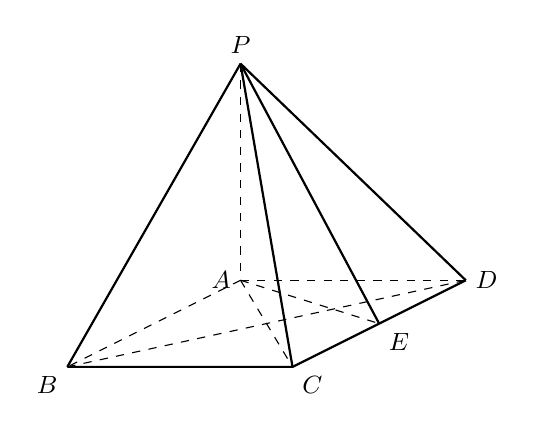
\begin{tikzpicture}[>=latex, font=\small, scale=1.1]
  \coordinate (A) at (0, 0);
  \coordinate (P) at (0, 2.5);
  \coordinate (B) at (-2.0, -1.0);
  \coordinate (D) at (2.6, 0);
  \coordinate (C) at (0.6, -1.0);
  \coordinate (E) at (1.6, -0.5);

  % 虚线：不可见棱与辅助线
  \draw[dashed, thin] (P) -- (A);
  \draw[dashed, thin] (A) -- (B);
  \draw[dashed, thin] (A) -- (D);
  \draw[dashed, thin] (A) -- (C);
  \draw[dashed, thin] (B) -- (D);
  \draw[dashed, thin] (A) -- (E);

  % 实线：可见棱与外轮廓
  \draw[thick] (B) -- (C) -- (D);
  \draw[thick] (P) -- (B);
  \draw[thick] (P) -- (C);
  \draw[thick] (P) -- (D);
  \draw[thick] (P) -- (E);

  % 顶点标签
  \node[above] at (P) {$P$};
  \node[left] at (A) {$A$};
  \node[below left] at (B) {$B$};
  \node[below right] at (C) {$C$};
  \node[right] at (D) {$D$};
  \node[below right] at (E) {$E$};
\end{tikzpicture}
\end{center}
\nopagebreak[4]
(1) 求证: $BD \perp$ 平面 $PAC$;

(2) 若 $\angle ABC = 60^\circ$, 求证: 平面 $PAB \perp$ 平面 $PAE$;

(3) 棱 $PB$ 上是否存在点 $F$, 使得 $CF \parallel$ 平面 $PAE$? 说明理由.

\end{question}
\begin{question}
\gkti{19}\textbf{（本小题满分 14 分）} 
已知椭圆 $C: \dfrac{x^2}{a^2} + \dfrac{y^2}{b^2} = 1$ 的右焦点为 $(1, 0)$, 且经过点 $A(0, 1)$.

(1) 求椭圆 $C$ 的方程;

(2) 设 $O$ 为原点, 直线 $l: y = kx + t$ ($t \neq \pm 1$) 与椭圆 $C$ 交于两个不同点 $P, Q$, 直线 $AP$ 与 $x$ 轴交于点 $M$, 直线 $AQ$ 与 $x$ 轴交于点 $N$, 若 $|OM| \cdot |ON| = 2$, 求证: 直线 $l$ 经过定点.

\end{question}
\begin{question}
\gkti{20}\textbf{（本小题满分 13 分）} 
已知函数 $f(x) = \dfrac{1}{4}x^3 - x^2 + x$.

(1) 求曲线 $y = f(x)$ 的斜率为 1 的切线方程;

(2) 当 $x \in [-2, 4]$ 时, 求证: $x - 6 \leqslant f(x) \leqslant x$;

(3) 设 $F(x) = |f(x) - (x + a)|$ ($a \in \mathbb{R}$), 记 $F(x)$ 在区间 $[-2, 4]$ 上的最大值为 $M(a)$. 当 $M(a)$ 最小时, 求 $a$ 的值.

\end{question}